%%%%%%%%%%%%%%%%%%%%%%%%%%%%%%%%%%%%%%%%%%%%%%%%%%%%%%%%%%%%%%%%%%%%%%%%%%%%%%%%%%%%%%%%%%%%%%%%%%%%%%%
% Sablona pro projekty ekonometrickych predmetu                                                     %%%
% Vytvoreno v ramci grantu: Ekonometricke nastroje a techniky v realnych ekonomickych aplikacich    %%%
% Autor: Jakub Bucek (jakubbucek@mail.muni.cz)                                                      %%%
% Pripominky, dotazy, namety smerujte na autora nebo na Daniela Nemce (danek@mail.muni.cz)		    %%%
% Vytvoreno: 1.12.2014                                                                              %%%
%%%%%%%%%%%%%%%%%%%%%%%%%%%%%%%%%%%%%%%%%%%%%%%%%%%%%%%%%%%%%%%%%%%%%%%%%%%%%%%%%%%%%%%%%%%%%%%%%%%%%%%

\documentclass[12pt,a4paper,oneside,final]{article}

%%%%%%%%%%%%%%%%%%%%%%%%%%%%%%%%%%%%%%%%%%%%%%%%%%%%%%%%%%%%%%%%%%%%%%%%%%%%%%%%%%%%%%%%%%%%%%%%%%%%%%%
%%%%%%%%%%%%%%%%%%%%%%%%%%%%%%%%%%%%%% ZAKLADNI NASTAVENI %%%%%%%%%%%%%%%%%%%%%%%%%%%%%%%%%%%%%%%%%%%%%

%% Nastaveni kodovani
\usepackage[utf8]{inputenc} 
\usepackage[IL2]{fontenc} %% fonty vhodne pro sazbu ceskych a slovenskych dokumentu
\usepackage[slovak]{babel}

\usepackage{subcaption}
\usepackage{float}

%% Fonty
\usepackage{mathptmx}  %% volne dostupny font Adobe Times Roman
% \usepackage{bookman}
% \usepackage{charter}
% \usepackage{fourier}
% \usepackage{mathpazo}
% \usepackage{newcent}
% \usepackage{palatino}
% \usepackage{utopia}

%% Baliky potrebne pro sazbu matematiky
\usepackage{amssymb,amsthm,amsmath}
\usepackage{bm}
\usepackage{tabularx} %% vylepsene tabulky

%% Balik nutny pro sablonu
\usepackage{garfield} %% nacteni stylu sablony

%% Vlastní definice
\renewcommand\vec[1]{\ensuremath\boldsymbol{#1}} %% tucne vektory
\newtheorem{veta}{Věta}[section]
\swapnumbers
\theoremstyle{definition}
\newtheorem{definice}{Definice}
\theoremstyle{remark}
\newtheorem*{pozn}{Poznámka}
\numberwithin{equation}{section}


\usepackage{xparse}
  \NewDocumentCommand{\INTERVALINNARDS}{ m m }{
      #1 {,} #2
 }

\NewDocumentCommand{\interval}{ s m >{\SplitArgument{1}{,}}m m o }{
      \IfBooleanTF{#1}{
          \left#2 \INTERVALINNARDS #3 \right#4
      }{
          \IfValueTF{#5}{
              #5{#2} \INTERVALINNARDS #3 #5{#4}
          }{
              #2 \INTERVALINNARDS #3 #4
          }
      }
  }

%%%%%%%%%%%%%%%%%%%%%%%%%%%%%%%%%%%%%%%%%%%%%%%%%%%%%%%%%%%%%%%%%%%%%%%%%%%%%%%%%%%%%%%%%%%%%%%%%%%%%%%
%%%%%%%%%%%%%%%%%%%%%%%%%%%%%%%%%%%%%%%% TITULNI STRANA %%%%%%%%%%%%%%%%%%%%%%%%%%%%%%%%%%%%%%%%%%%%%%%

\NazevPrace{Modelovanie časových radov z monitorovacieho systému Hawkular}
\Autor{Bc. Pavol Loffay}
\Univerzita{Masarykova univerzita}
\Fakulta{Fakulta informatiky}
\Obor{Service Science Management Engineering}
\Mail{p.loffay@mail.muni.cz}
\DatumOdevzdani{\today}
\Abstrakt{
 Práca spracováva predikciu časových radov prevziatych z monitorovacieho systému
 Hawkular\footnote{Dostupné na \url{http://www.hawkular.org}}. Tento systém dokáže
 monitorovať Java aplikácie, alebo fyzický hardvér na ktom je spustený.
 Z množiny pozorovaných metrík bola vybratá vyťaženosť Java hromady (heap).
 Pre túto časovú rady boli zostrojené modeli: \emph{ARIMA} a exponenciálne vyhladzovanie.
 Bola demonštrovaná adaptívna filtrácia pomocou algoritmu \emph{LMS} na výpočet
 koeficientov \emph{AR} modelu na generovaných dátach.
}
\KlicovaSlova{Časová rada; ARIMA; LMS; Exponenciálne vyhladzovanie; Hawkular;}
\JELklasifikace{C53}

%%%%%%%%%%%%%%%%%%%%%%%%%%%%%%%%%%%%%%%%%%%%%%%%%%%%%%%%%%%%%%%%%%%%%%%%%%%%%%%%%%%%%%%%%%%%%%%%%%%%%%%
%%%%%%%%%%%%%%%%%%%%%%%%%%%%%%%%%%%%%% ZACATEK DOKUMENTU %%%%%%%%%%%%%%%%%%%%%%%%%%%%%%%%%%%%%%%%%%%%%%

\begin{document}
\VytvorTitulniStranu

\section{Úvod}
Monitorovanie doležitých business aplikácii medzi ktoré napríklad patria bankové systémy alebo rôzne
servery, na ktorých bežia služby ktoré sú využívané 24/7 je veľmi dôležité. Vačšina
monitorovacích systémov dokáže upozorniť administrátora na vyťaženie pri prekročení
hraničnej hodnoty. V monitorovacom systéme Hawkular je možné zapnúť predikciu, takže
administrátor bude upozornený vopred ak by náhodov malo dôjsť k prekročeniu spomenutej
hraničnej hodnoty. Použíté modely časových rád v systéme Hawkular sú varianty
exponenciálneho vyhladzovania. Modely \emph{ARIMA} nemohli byť použité z dôvodu nestacionarity dát 
a náročnosti na výpočet\,--\,systém je schopný analyzovať aj niekoľko tisíc model naraz. 

Táto práci sa zameria na konštrukciu optimálneho \emph{ARIMA} modelu, ktorý následne porovná
s exponenciálnym vyhladzovaním konkrétne Holtovou metódou s linárnym trendom. Následne
bude demonštrovaná adaptívna filtrácia. Pre výpočetnú nenáročnosť  bola použitá 
kombinácia exponenciálneho vyhladzovania a
adaptívnej filtrácie v sýstéme Hawkular.


\section{Identifikácia ARIMA modelu}
V tejto kapitole budeme analyticky identifikovať najvhodnejší \emph{ARIMA} model, ktorý následne 
porovnáme s výsledom funkcie \texttt{auto.arima} z balíka \texttt{forecast} v jazyku
\emph{R}.

Začneme vykreslením časovej rady. Na obrázku \ref{obr:heap} je možné vidieť, že časová rada 
obsahuje mierny lineárny trend, čo indikuje nestacionaritu. Vykresíme autokorelačnú 
(zkrátene \emph{ACF}) a parciálknu autokorelačnú funkciu (zkrátene \emph{PACF}).

\begin{figure}[H] 
    \begin{center}
        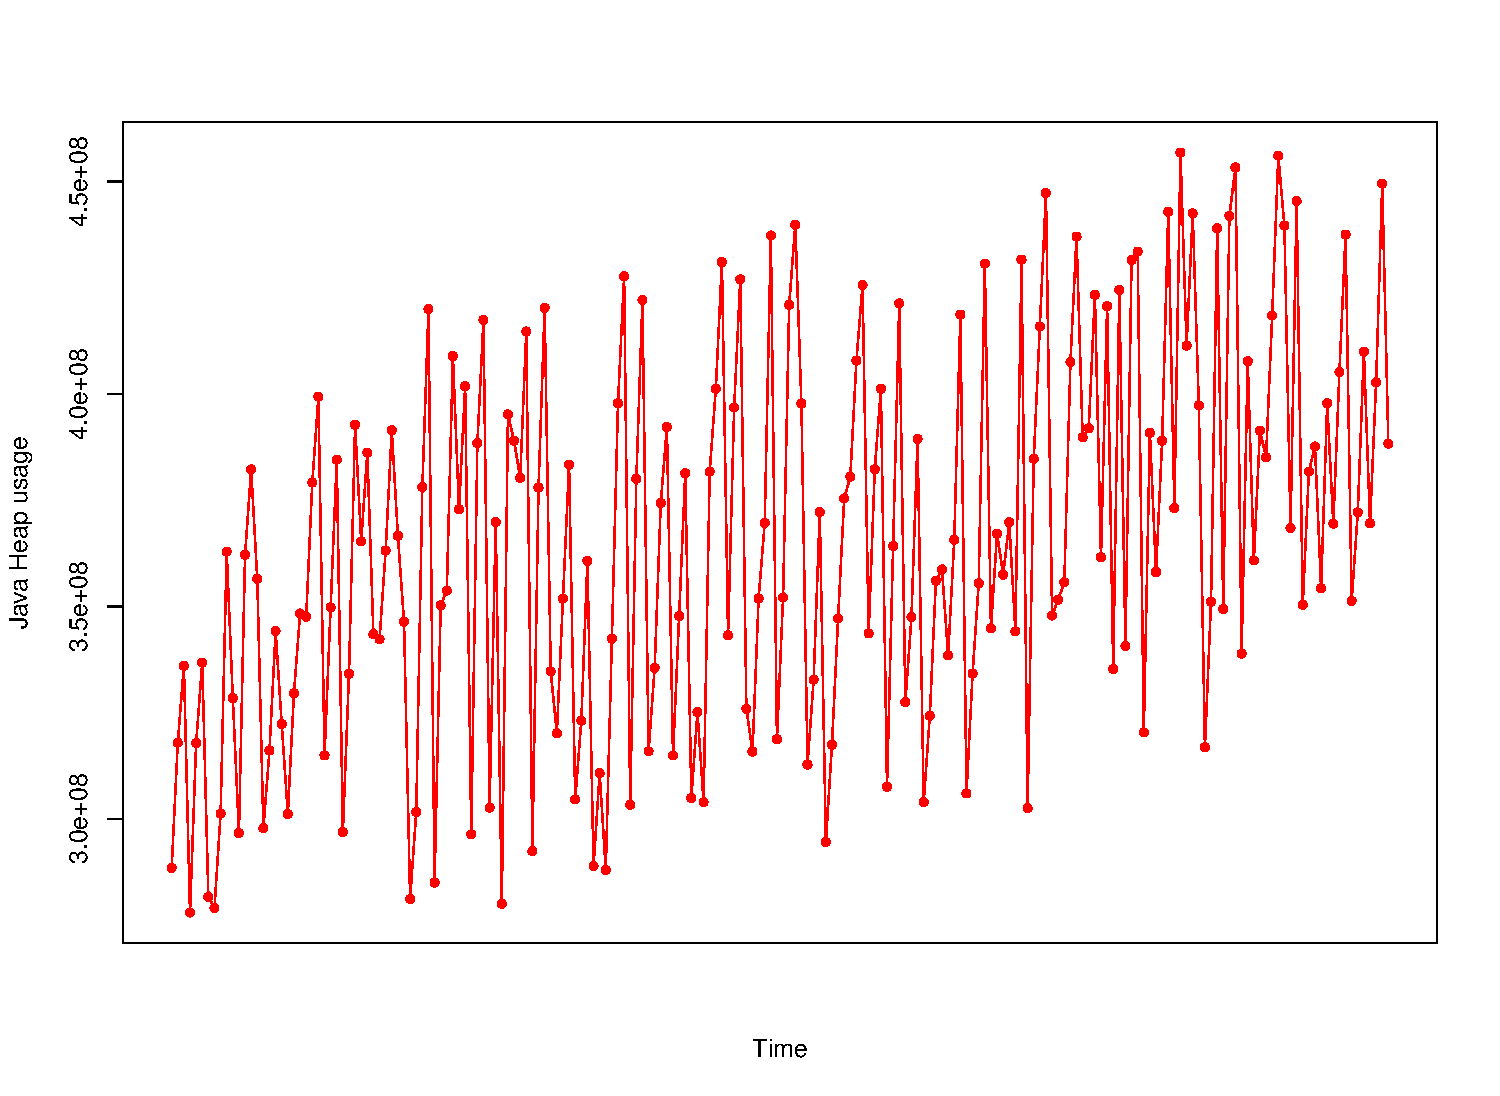
\includegraphics[width=.8\textwidth]{images/heap_series.pdf}
        \caption{Vyťaženosť Java Heap-u v čase.}
        \label{obr:heap} % unikatni navesti, pomoci ktereho se budeme v textu odvolavat na dany obrazek
    \end{center}
\end{figure}

\begin{figure}[H] \centering
    \begin{subfigure}[b]{0.45\textwidth}
        \centering
        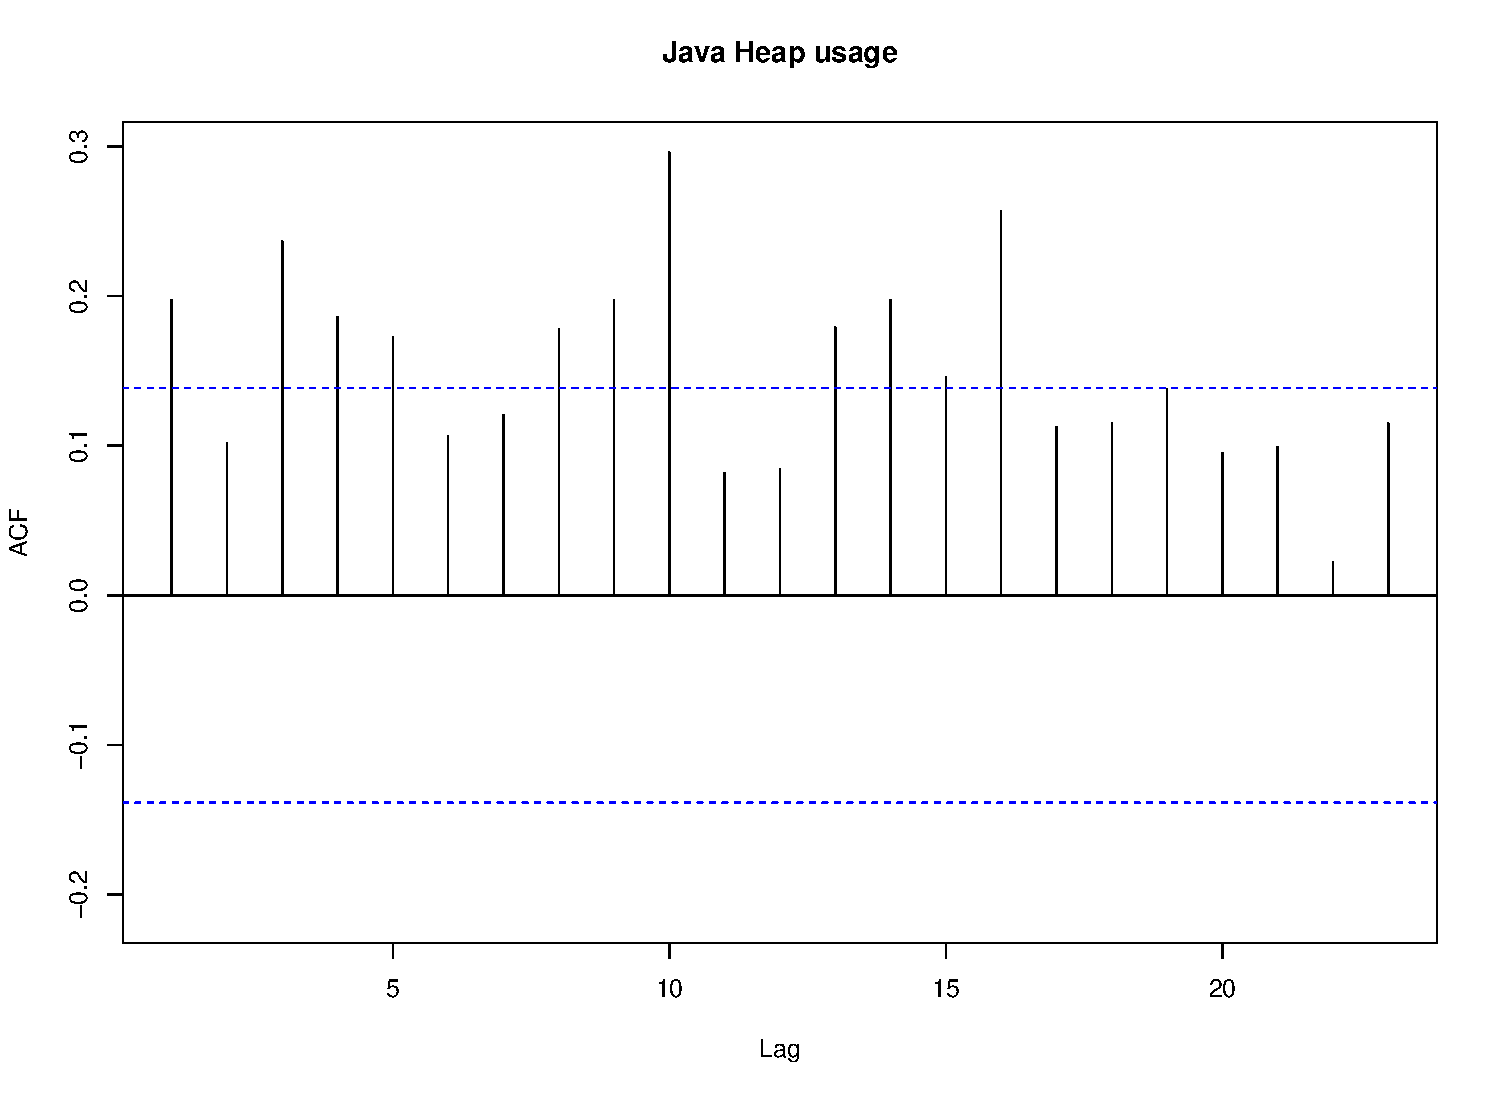
\includegraphics[width=1\linewidth]{images/heap_acf.pdf}
        \caption{Autokorelačná funkcia.}
        \label{obr:heap_acf}
    \end{subfigure}
    \begin{subfigure}[b]{0.45\textwidth}
        \centering
        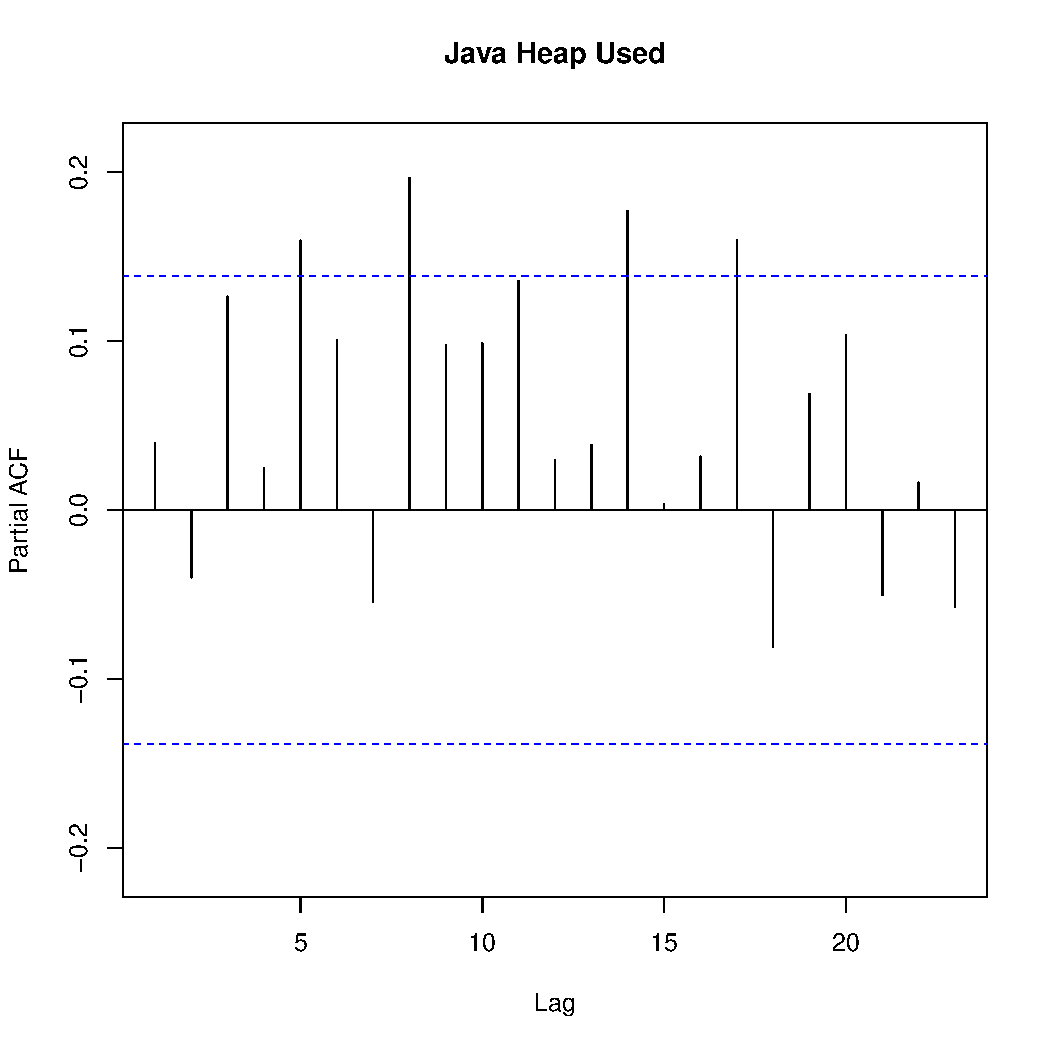
\includegraphics[width=1\linewidth]{images/heap_pacf.pdf}
        \caption{Parciálna autokorelačná funkcia.}
        \label{obr:heap_pacf}
    \end{subfigure}
%    \caption{Parciálna autokorelačná funkcia.}
    %\label{fig:test}
\end{figure}

Z grafu autokorelačnej funkcie \ref{obr:heap_acf} je vidieť že hodnoty sú kladné,
relatívne blízko nuly a neklesajú. 
Na grafe \emph{ACF} taktiež nie sú prítomné periodicky posunuté vysoké hodnoty, 
ktoré by indikovali sezónnosť.
Keďže hodnoty \emph{ACF} so zvyšujúcim spozdením neklesajú k nule rozhodli sme sa urobiť
\emph{ADF} test na testovanie stacionarity.

\begin{minipage}{\linewidth}
\begingroup
\fontsize{9pt}{7pt}\selectfont  %ADF
\begin{verbatim}
> adfTest(heap, lags = 0, type='nc');
Title:
 Augmented Dickey-Fuller Test
Test Results:
  PARAMETER:
    Lag Order: 0
  STATISTIC:
    Dickey-Fuller: -1.1436
  P VALUE:
    0.2508 
\end{verbatim}
\endgroup
\end{minipage}

Nulovú hypotézu \emph{ADF} testu o prítomnosti jednotkového koreňa, na hladine významnosti 0.05
nezamietame. Z toho vyplýva, že naša časová rada je nestacionárna. Pre dôkladné 
overenie skusíme \emph{KPSS} test, ktorého nulová hypotéza znie, že časová rada je stacionárna.

\begin{minipage}{\linewidth}
\begingroup
\fontsize{9pt}{7pt}\selectfont %KPSS
\begin{verbatim}
> kpss.test(heap);
	KPSS Test for Level Stationarity
data:  heap
KPSS Level = 2.1652, Truncation lag parameter = 3, p-value = 0.01
\end{verbatim}
\endgroup
\end{minipage}

Na hladine významnosti 0.05 by sme nulovú hypotézu zamietli. Oba testy nám ukázali, že časová
rada nie je stacinárna. 
Následne môžeme pomocou \emph{KPSS} testu testovať či je daná časová rada trend stacinárna.

\begin{minipage}{\linewidth}
\begingroup
\fontsize{9pt}{7pt}\selectfont %KPSS Trend
\begin{verbatim}
> kpss.test(heap, null='Trend');
	KPSS Test for Trend Stationarity
data:  heap
KPSS Trend = 0.087693, Truncation lag parameter = 3, p-value = 0.1

> ndiffs(heap)
[1] 1

> diff = diff(heap)
\end{verbatim}
\endgroup
\end{minipage}

Z výstupu je jasné, že rada je trend stacinárna takže nulovú hypotézu na hladine 0.05
nezamietame.

Časovú radu stacionarizijeme diferenciovaním a pokračujeme vykreslením \emph{ACF} a
\emph{PAC} upravenej časovej rady. 
Významny bod useknutia sa nám v oboch grafoch \ref{obr:heap_diff_acf_pacf} nepodarilo nájsť. 
To indikuje, že výsledny 
model sa bude skladať z \emph{AR} aj \emph{MA} zložky. Teraz by sme mali hľadať krivku 
\emph{U}, ktorá od nejakého bodu pripomína krivku v tvare linearnych kombinácii klesajúcich
geometrických postupností sinusoid s geometricky klesajúcimi amplitudami.
Túto krivka v grafe \emph{ACF} ani \emph{PACF} nie je jednoznačne prítomná \ref{cipra}. 
Rozhodli sme sa vybrať model \emph{ARIMA(2,1,1)}. Do modelu sme zahrnuli dve najväčšie 
hodnoty \emph{PACF} (model \emph{AR}) a jednu \emph{ACF} (model \emph{MA})

\begin{figure}[H] \centering
    \begin{subfigure}[b]{0.45\textwidth}
        \centering
        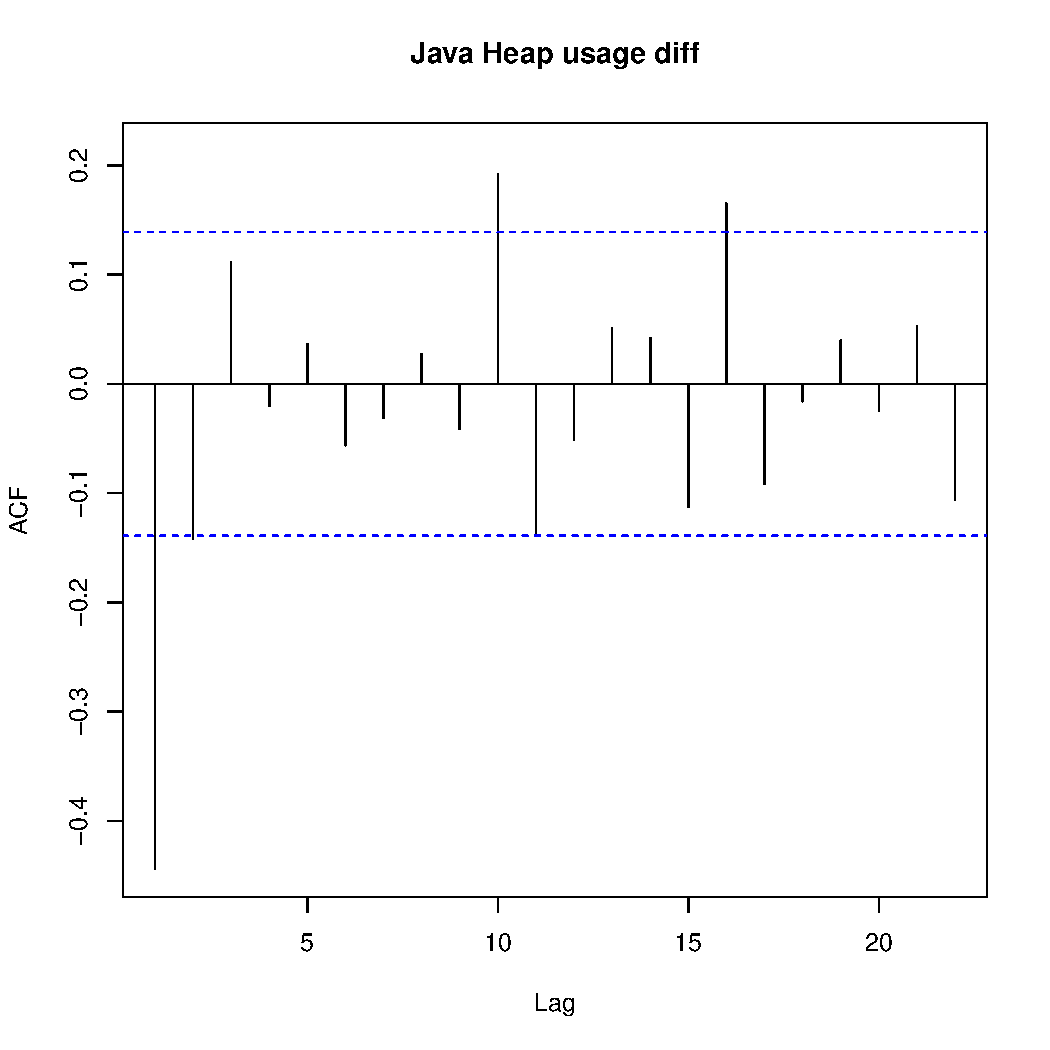
\includegraphics[width=1\linewidth]{images/heap_diff_acf.pdf}
%        \caption{Autokorelačná funkcia diferencovanej rady.}
%        \label{obr:heap_diff_acf}
    \end{subfigure}
    \begin{subfigure}[b]{0.45\textwidth}
        \centering
        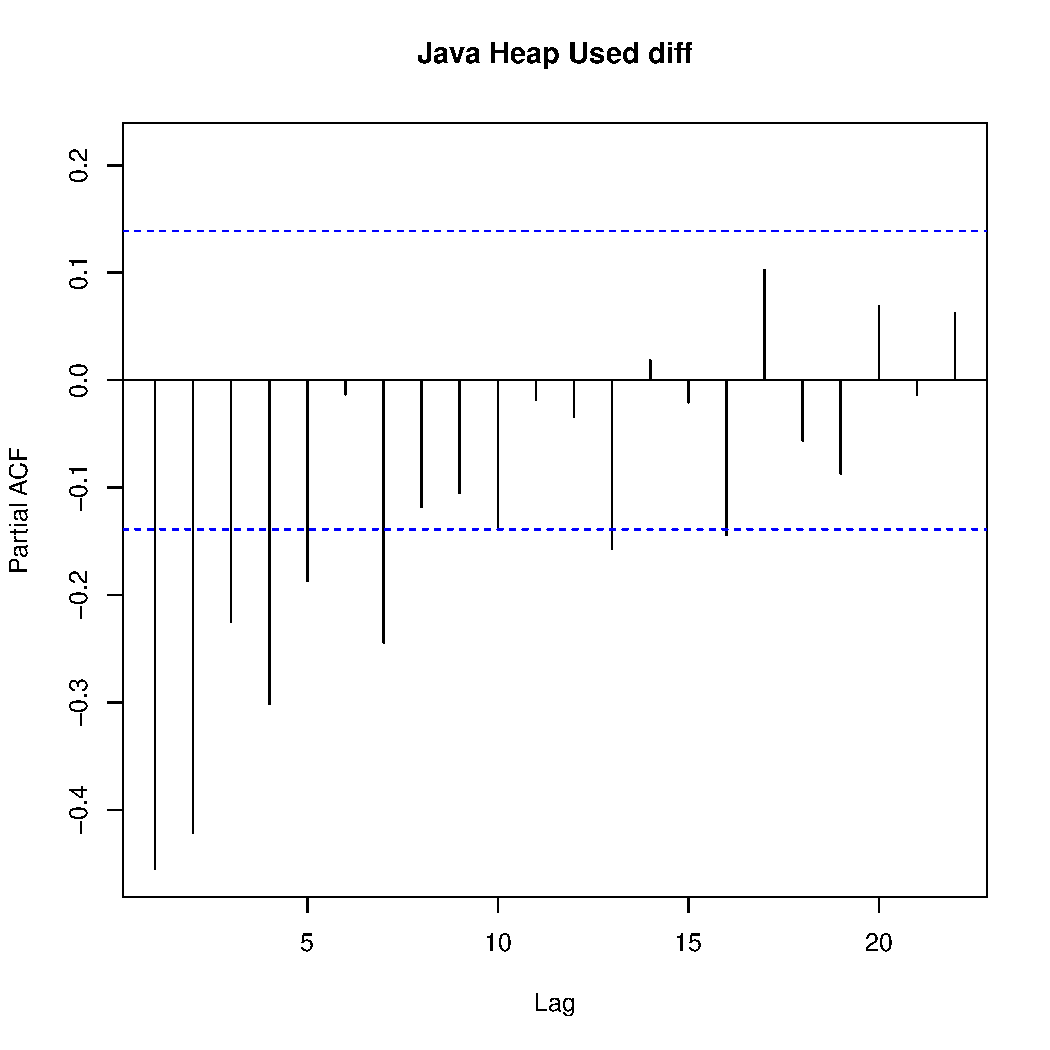
\includegraphics[width=1\linewidth]{images/heap_diff_pacf.pdf}
%        \caption{Parciálna autokorelačná funkcia diferencovanej rady.}
%        \label{obr:heap_diff_pacf}
    \end{subfigure}
    \caption{ACF a PACF diferencovanej časovej rady.}
    \label{obr:heap_diff_acf_pacf}
\end{figure}

Alternatívny spôsob voľby modelu je pomocou informačných kritérii. Tento spôsob je
vhodný pre plne automatizované spracovanie \cite{cipra} napríklad v ekonometrických 
softvéroch. K identifikácia modelu \emph{ARMA(p, q)} sa pristupuje ako k minimalizácii funkcie
\ref{rov:inf_k}.

\begin{eqnarray} \label{rov:inf_k}
    (\hat{p}, \hat{q}) =arg\ \underset{(k,l)}{min}\ A(k, l)
\end{eqnarray}

\emph{A} je vhodné kritérium pre výpočet ktorého musíme odhadnúť model
\emph{ARMA(k,l)}. Pri minimalizácii postupne inkrementujeme oba parametre k, l.
Informačných kritérii existuje viac. V tejto práci sme zvolili Akaikeho informačné kritérium:

\begin{eqnarray} \label{rov:aic}
    A(k,l) = AIC(k,l) = ln\hat{\sigma}^{2}_{k,l} + \frac{2(k+l+1)}{n}
\end{eqnarray}

Z rovnice \ref{rov:aic} je zrejmé, že kritérium penalizuje veľké rády k a l. 
$\hat{\sigma}^{2}_{k,l}$ je smerodajná odchylka reziduí modelu. 
Poďme si vypísať niekoľko kandidátov \emph{ARIMA} modelov pomocu príkazu auto.arima().

\begin{minipage}{\linewidth}
\begingroup
\fontsize{9pt}{7pt}\selectfont %ARIMA
\begin{verbatim}
> auto.arima(diff, approximation=FALSE, trace=TRUE, ic='aic', allowdrift=FALSE)
 ARIMA(2,1,2)                    : 7556.055
 ARIMA(0,1,0)                    : 7696.058
 ARIMA(1,1,0)                    : 7651.407
 ARIMA(0,1,1)                    : 7557.045
 ARIMA(1,1,2)                    : 7560.654
 ARIMA(3,1,2)                    : 7557.714
 ARIMA(2,1,1)                    : 7553.937
 ARIMA(1,1,1)                    : 7557.937
 ARIMA(3,1,1)                    : 7555.879
 ARIMA(2,1,0)                    : 7613.902

 Best model: ARIMA(2,1,1)                    
Series: diff 
ARIMA(2,1,1)                    
Coefficients:
          ar1      ar2      ma1
      -0.0985  -0.1774  -0.9441
s.e.   0.0716   0.0716   0.0199
\end{verbatim}
\endgroup
\end{minipage}

Ako je vidieť funkcia zvolila model \emph{ARIMA(2,1,1)} ktorého \emph{AIC} kritérium bolo najnižšie.
Odhadnutý model môžeme zapísať v tvare:
\begin{eqnarray} \label{rov:arima_model}
    Y_t = -0.985 Y_{t-1} - 0.1774 Y_{t-2} -0.9441\epsilon_{t-1} + \epsilon_{t}
\end{eqnarray}

Ukázali sme, že je možné konštrulovať správny \emph{ARIMA} model aj analytickým spôsobom. 
Chcel by som avšak poznanenať, že voľbu modelu je lepšie prenechať overenému 
štatistickému softvéru. 

Po úspšnom odhade rádu modelu je by sme chceli zmieniť ako sa počítajú jednotlivé
koeficienty. Pre \emph{AR} model platí, že sa dajú vypočítať pomocou \emph{OLS} alebo Yule\,--\,Walkerových
rovníc \cite{brockwell_ts}. Výpočet kofeicientov \emph{MA} modelu je zložitejší a 
je možný pomocou rekurzívnej Levison-Durbin metódy.
Odhadom presných parametrov modelu sa v tejto práci ďalej nebudene zaoberať.  

Na záver sa pozrieme na rezíduá odhadnutého modelu. Ak sme postupovali správne rezíduá by
mali pripomínať biely šum a nemali by byť korelované (inakšie by sme ich
vedeli modelovať). Toto tvrdenie si overíme Ljung\,--\,Box testom, ktorého nulová hypotéza
hovorí o tom, že dáta sú nezávislé distribuované. Z grafu \ref{obr:heap_resid} môžeme
prehlásiť, že nulovú hypotézu na hladine významnosti 0.05 nezamietame.

Na následujúcich grafoch si vykresíme rezíduá modelu, ich autokorelačnú funkciu a p-hodnoty
pre rôzdne opozdenia Ljung\,--\,Box testu.

\begin{figure}[H] \centering
    \begin{subfigure}{0.55\textwidth}
        \centering
        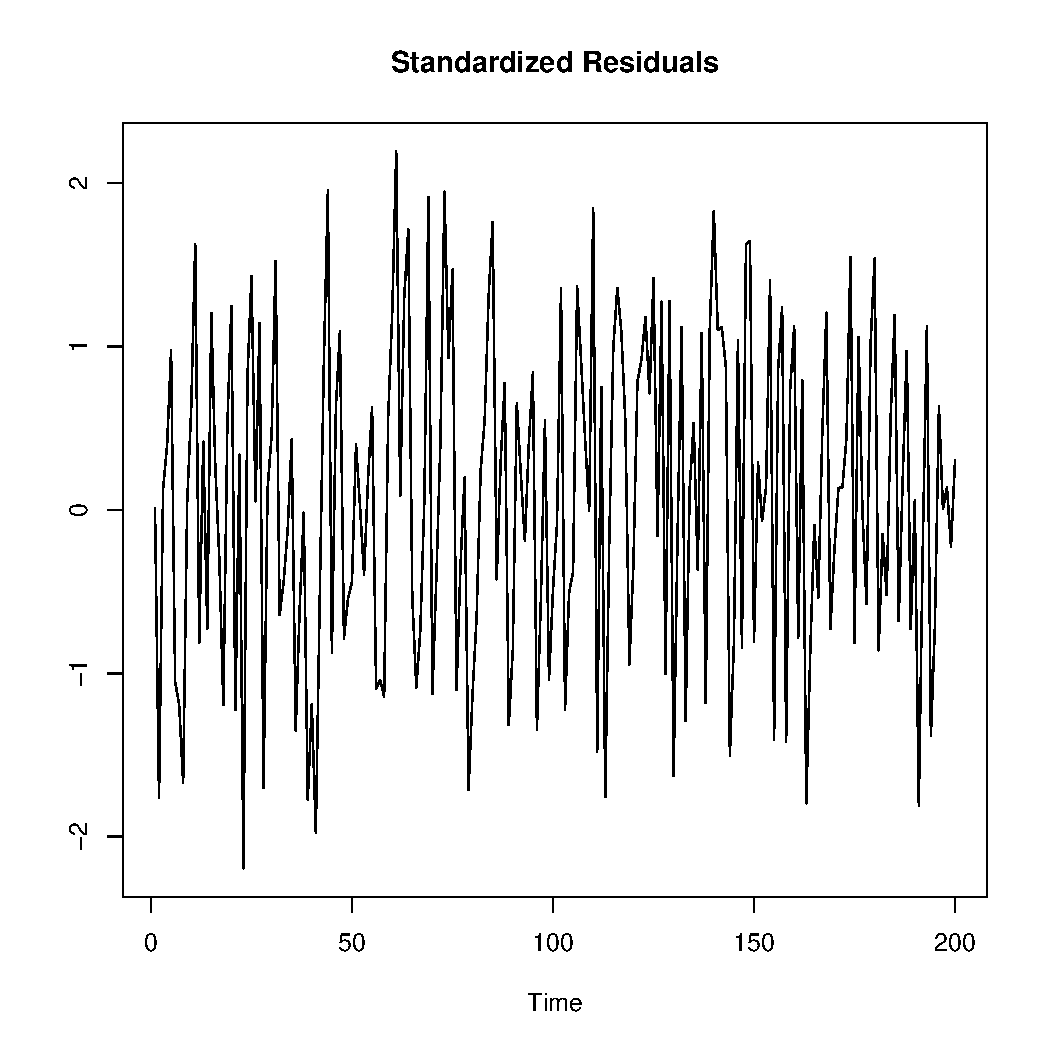
\includegraphics[width=1\linewidth,height=5cm]{images/heap_resid.pdf}
%        \caption{}
        \label{obr:heap_resid_resid}
    \end{subfigure}
    \begin{subfigure}{0.55\textwidth}
        \centering
        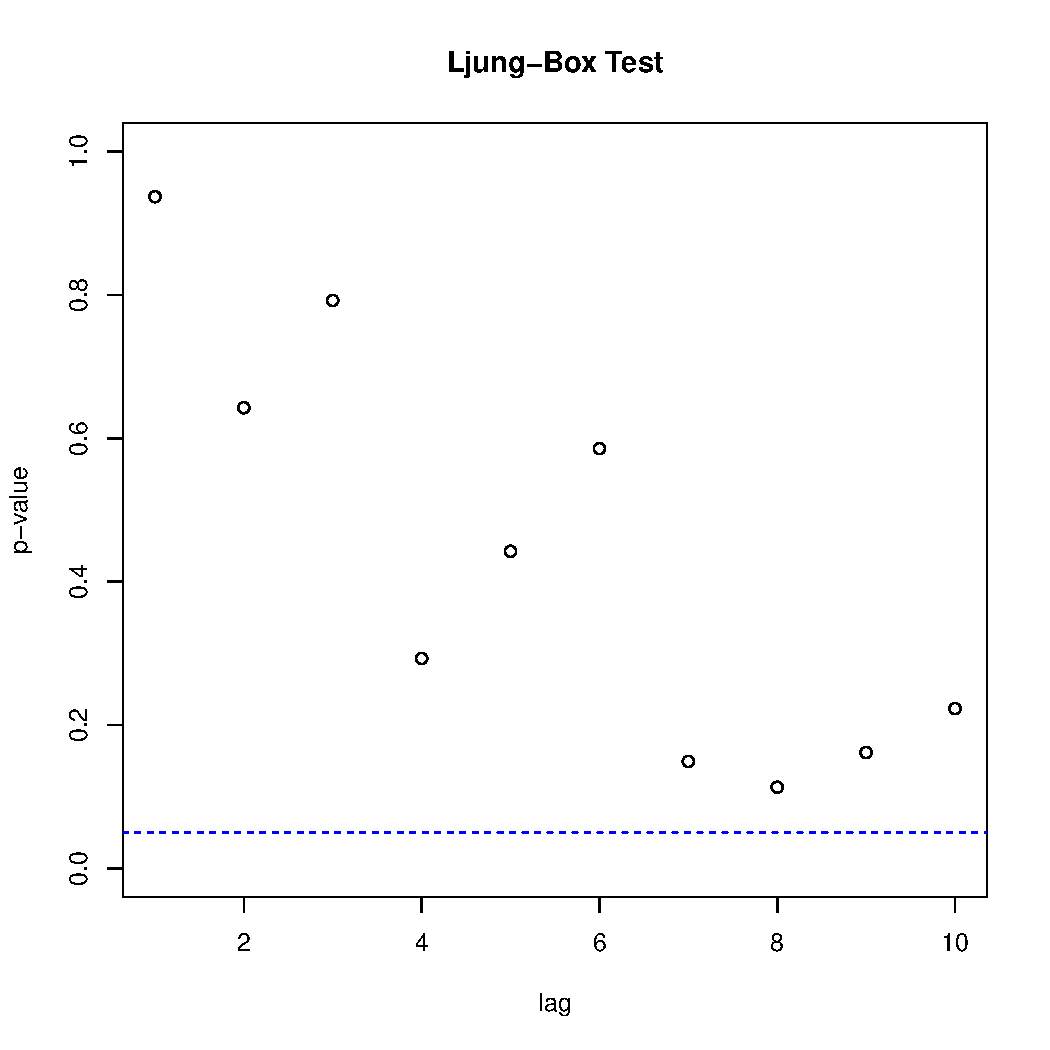
\includegraphics[width=1\linewidth,height=5cm]{images/heap_box.pdf}
%        \caption{}
%        \label{obr:heap_resid_ljung}
    \end{subfigure}
    \caption{Rezíduá odhadnutého \emph{ARIMA} modelu.}
     \label{obr:heap_resid}
\end{figure}

\begin{figure}[H]
    \begin{center}
        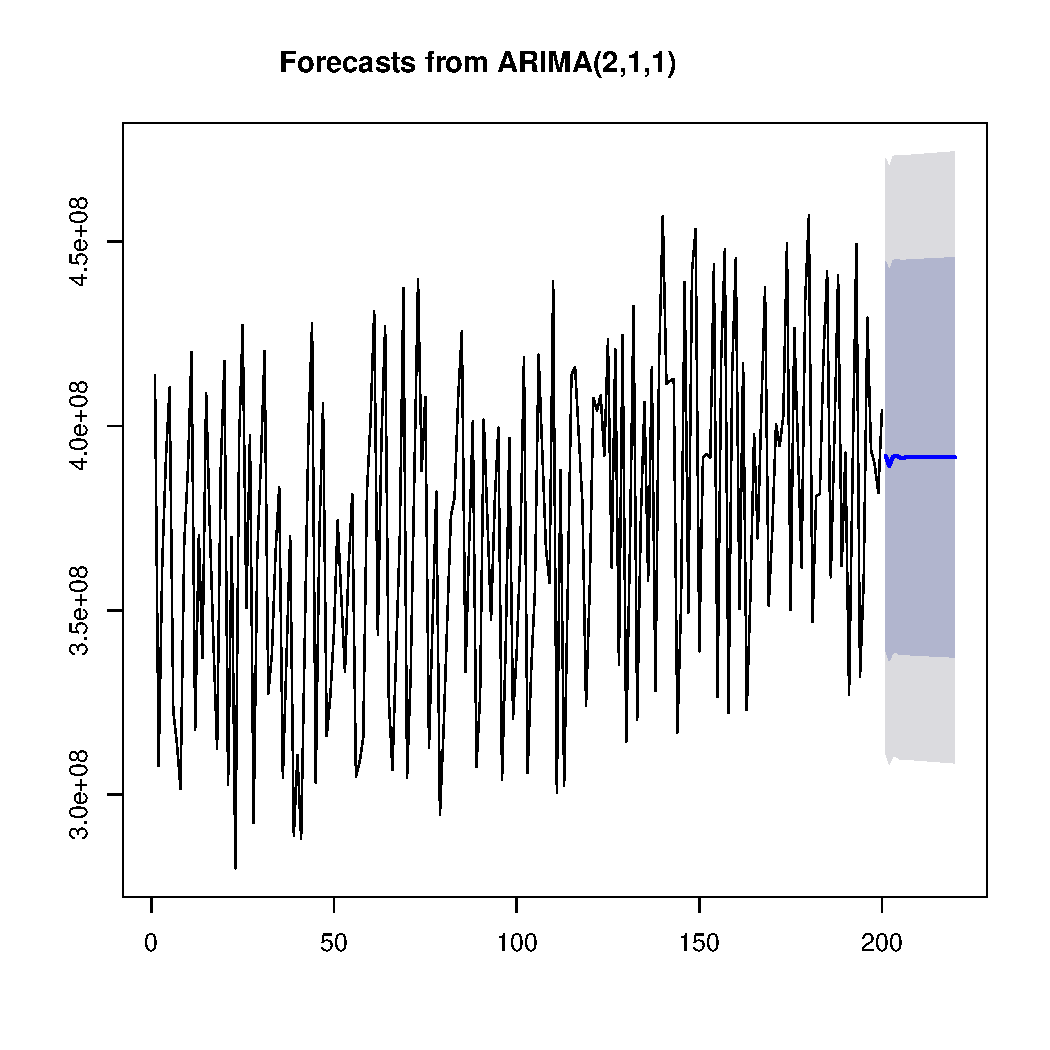
\includegraphics[width=.8\textwidth,height=6cm]{images/heap_forecast.pdf}
        \caption{ARIMA, predikcia na 20 krokov do predu.}
        \label{obr:heap_forecast}
    \end{center}
\end{figure}

\section{Exponenciálne vyhladzovanie\,--\,Holtova metóda}
Zobecnením dvojitého exponenciálneho vyhladzovania je takzvaná Holtova metoda.
Táto metóda používa dve vyrovnávacie konštanty: $\alpha$ pre vyrovnanie úrovne $l_t$
a $\beta$ pre vyrovnanie smernice $b_t$ (lineárneho trendu).
Výhoda tejto metódy je možnosť použitia v prúdovom spracovaní, kde nie je možné získať staré hodnoty časovej rady. 
Rovnice majú tvar \ref{exp_holt}. Parametre $\alpha, \beta$ patria do intervalu 
$\alpha,\beta \in (0,1)$. Pre exponenciálne vyhladzovanie platí, 
čím je hodnota parametra $\alpha$ menšia, tak väčšia váha je daná pozorovaniam z
vzdialenej minulosti.

\begin{eqnarray} \label{exp_holt}
    \hat{y}_{t+h} = l_{t} + hb_{t} \\
    \nonumber l_t = \alpha y_t + (1 - \alpha) (l_{t-1} + b_{t-1}) \\
    \nonumber b_t = \beta (l_t - l_{t-1}) + (1 - \beta)b_{t-1} 
\end{eqnarray}
 
V jazyku \emph{R} použijeme funkciu \emph{holt}, ktorá počíta predikciu na \emph{k} krokov 
do predu. Súčasťou funkcie je aj výpočet parametrov $\alpha$ a $\beta$.

\begin{figure}[H]
    \begin{center}
        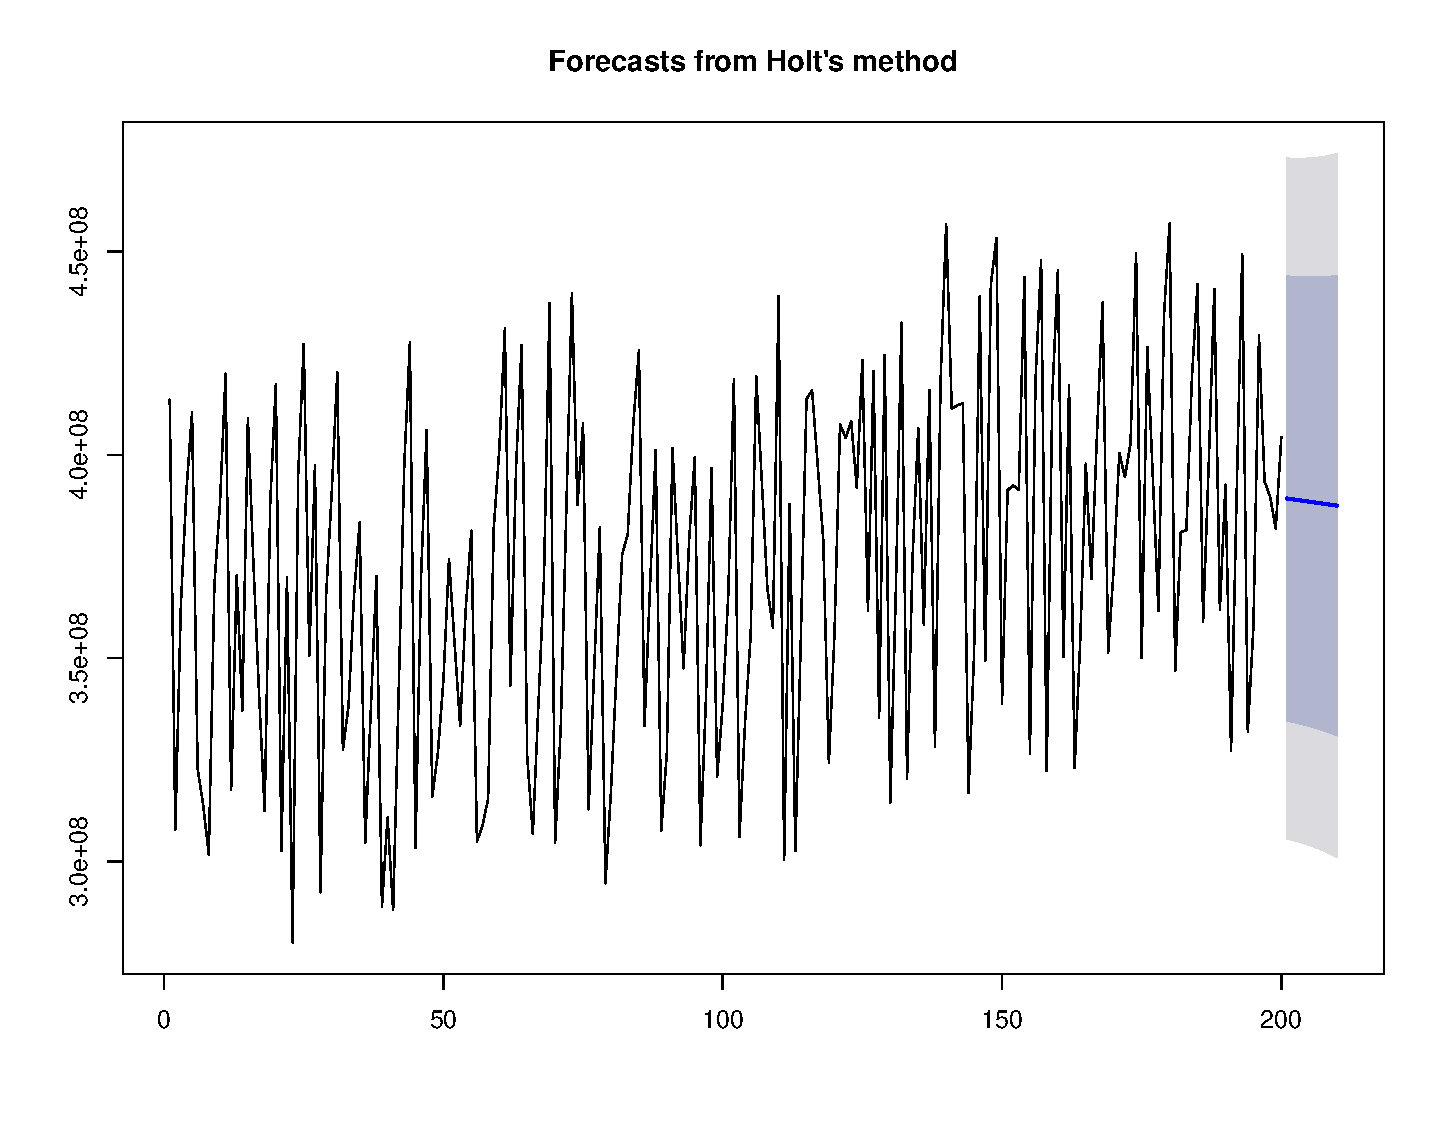
\includegraphics[width=.8\textwidth,height=6cm]{images/heap_holt.pdf}
        \caption{Holt, predikcia na 20 krokov do predu.}
        \label{obr:heap_holt}
    \end{center}
\end{figure}

\section{Adaptívna filtrácia\,--\,LMS algoritmus}
Odhad parametrov autoregresívneho modelu je možné vypočítať 
pomocou algoritmu \emph{LMS} (Least Mean Square). Výpočet venktoru váh je uvedený v
rovnici \ref{lms}. Chyba $e$ je rozdiel súčasnej hodnoty časovej rady s odhadnutov pomocou
váh \emph{LMS}. S väčším počtom pozorovaní je výpočet váh presnejší. Algoritmus 
má nevýhodu, že dopredu musíme odhanúť parameter $\alpha$. Toto býva väčšinou problém 
a preto sa volí buď normalizovaná verzia algoritmu alebo algoritmus RLS (Recursive Least
Square) pri ktorý tento parameter neobsahuje. V porovnaní RLS algoritmus konverguje
rýchlejšie ale je výpočetne náročnejsí.  

\begin{eqnarray} \label{lms}
    w(t+1) = w(t) + \alpha * e(t) * x(t)
\end{eqnarray}

Funkčnosť algoritmu budeme demonštrovat na gererovaných dátach, pri ktorých vieme 
aký proces ich generoval. Takto budeme môcť výsledky overiť s výstupom s \emph{LMS} algoritmu.

\begin{minipage}{\linewidth}
\begingroup
\fontsize{9pt}{7pt}\selectfont
\begin{verbatim}
n = 1500;
series = arima.sim(n, model=list(ar=c(0.3, -0.8745)), rand.gen=rnorm);
result = lms(series, alpha, AR);
"Estimated weights"
[1]  0.3397577 -0.8287951
\end{verbatim}
\endgroup
\end{minipage}

Z uvedeného výstupu z R vidíme že časová rada bola generovaná pomocou
$y = 0.3*y_{t-1} - 0.8745*y_{t-2}$ a na vstup vstup dát z normálneho rozdelenia so
strednou hodnotou 0 a smerodatnou odchylkou 1. Z grafu \ref{obr:lms} je vidieť priebeh
výpočtu váh pomocou \emph{LMS} algoritmu.

\begin{figure}[H]
    \begin{center}
        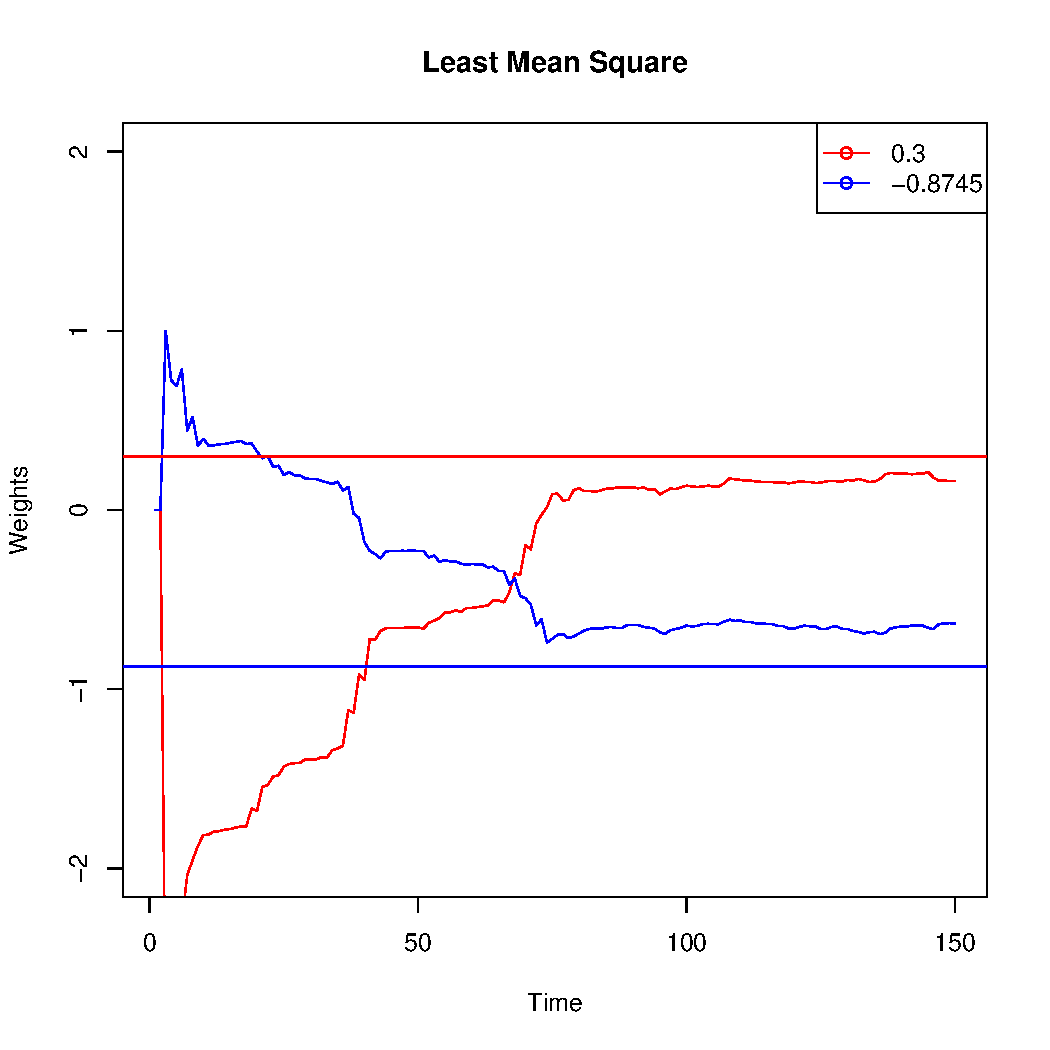
\includegraphics[width=.8\textwidth,height=6cm]{images/lms.pdf}
        \caption{Priebeh výpočtu váh AR procesu pomocu LMS algoritmu.}
        \label{obr:lms}
    \end{center}
\end{figure}

\section{Záver}
Na záver by som porovnal kvadratickú sumu chýb (\emph{SSE}) oboch modelov. Pre
model \emph{ARIMA} chyba vyšla $3.377059*10^17$ pre Holtovu metódu $3.657135*10^17$. 
Vidíme, že rozdiel nieje významne iný. Keď opticky porovnáme grafy \ref{obr:heap_forecast},
\ref{obr:heap_holt} vidíme, že exponenciálne vyhladzovanie strmšie klesá.

Voľba vhodnéh modelu niekedy nezávisi len na najmenšej chybe predpovedi. Niekedy je nutné
voliť výpočetne nenáročny model, aby bolo napríklad možné spracovávať obrovské množstvo 
časových rád paralelne.

Výsledky adaptívnej filtrácie ukázali, že je možná vypočítať parametre \emph{AR} modelu
pomoocu jednoduchých algoritmov ako je napríklad \emph{LMS} ak máme dostatočne veľký počet
pozorovaní. Kombináciou adaptívnej filtrácie a exponenciálneho vyhladzovania by sme mohli 
dospieť k zaujímavému modelu, ktorý by mohol mať odbré prediktívne vlastnosti a nízku
výpočetnu náročnosť.

\section*{Poďakovanie}
Na záver by som chcel poďakovať Ing. Danielovi Němcovi, Ph.D. za návrh na vypracovanie
tejto témi a za veľmi príjemné a užitočné konzultácie. Ďalej by som chcel poďakovať Ester
Železňákovej za gramatickú korektúru textu.

\bibliographystyle{czechiso}
\bibliography{bibliography}

%% Pokud nechcete pouzit prilohy, muzete nasledujici radky az po \end{document} smazat
\newpage
\renewcommand{\thesection}{\Alph{section}}
\setcounter{section}{0}
\renewcommand{\thepage}{\roman{page}}
\setcounter{page}{1}

\section{Prílohy}

\begin{itemize}
    \item Zdrojové súbory v jazyku R v adresáry \texttt{scripts}
    \item Dáta analyzovanej časovej rady v adresáry \texttt{scripts}
    \item Zdrojový text tejto správy v \LaTeX\,--\,e
\end{itemize}

\end{document}

